\documentclass[aspectratio=169]{beamer}

\mode<presentation>
\usetheme{Boadilla}
\definecolor{redback}{RGB}{140,0,0}
\definecolor{blue}{RGB}{30,90,205}
\definecolor{red}{RGB}{213,94,0}
\definecolor{green}{RGB}{0,128,0}
\setbeamercolor{title}{fg=redback}
\setbeamercolor{frametitle}{fg=redback}
\setbeamercolor{block title}{bg=redback, fg=white}
\setbeamercolor{block body}{bg=white}
\setbeamercolor{structure}{fg=redback}
\setbeamercolor{item projected}{fg=white}
\setbeamercolor{item}{fg=redback}
\setbeamercolor{subitem}{fg=redback}
\setbeamercolor{section in toc}{fg=redback}
\setbeamercolor{description item}{fg=redback}
\setbeamercolor{caption name}{fg=redback}
\setbeamercolor{button}{bg=redback, fg=white}
\setbeamercolor{caption name}{fg=redback}
\usepackage{graphics}
\usepackage{tikz}
\usepackage{amsmath}
\usepackage{bbm}
\usetikzlibrary{decorations.pathreplacing}
\usepackage{geometry}
\usepackage{booktabs}
\usepackage{multirow, makecell}
\usepackage{float}
\usepackage{fancyvrb}
\usepackage{kotex}
\usepackage{caption}
\usepackage{subcaption}
\usepackage{adjustbox}
\usepackage{hyperref}
\usepackage{threeparttable}
\usepackage[scaled=0.92]{helvet}
\usepackage[default]{lato} %If I want a twist
\newenvironment{wideitemize}{\itemize\addtolength{\itemsep}{10pt}}{\enditemize}
\newenvironment{wideenumerate}{\enumerate\addtolength{\itemsep}{10pt}}{\endenumerate}
\newenvironment{widedescription}{\description\addtolength{\itemsep}{10pt}}{\enddescription}
\hypersetup{
colorlinks=true,
linkcolor=redback,
filecolor=green, 
urlcolor=blue,
}
\beamertemplatenavigationsymbolsempty
\setbeamercolor{author in head/foot}{bg=white, fg=redback}
\setbeamercolor{title in head/foot}{bg=white, fg=redback}
\setbeamercolor{date in head/foot}{bg=white, fg=redback}
\setbeamercolor{section in head/foot}{bg=white, fg=redback}
\setbeamercolor{page number in head/foot}{bg=white, fg=redback}
\setbeamercolor{headline}{bg=redback}
\setbeamertemplate{footline}{
    \leavevmode%
    \hbox{%
        \begin{beamercolorbox}[wd=.333333\paperwidth,ht=2.25ex,dp=1ex,center]{date in head/foot}%
            \usebeamerfont{date in head/foot}\insertshortdate
        \end{beamercolorbox}%
        \begin{beamercolorbox}[wd=.444444\paperwidth,ht=2.25ex,dp=1ex,center]{title in head/foot}%
            \usebeamerfont{title in head/foot}\insertshorttitle
        \end{beamercolorbox}%
        \begin{beamercolorbox}[wd=.222222\paperwidth,ht=2.25ex,dp=1ex,center]{page number in head/foot}%
            \usebeamerfont{page number in head/foot} \insertframenumber{} / \inserttotalframenumber
        \end{beamercolorbox}}%
        \vskip0pt%
    }

\setbeamertemplate{section in toc}[sections numbered]
\setbeamertemplate{subsection in toc}{\leavevmode\leftskip=3em\rlap{\hskip-1.75em\inserttocsectionnumber.\inserttocsubsectionnumber}\inserttocsubsection\par}
\setbeamerfont{subsection in toc}{size=\footnotesize}

\newenvironment{transitionframe}{\setbeamercolor{background canvas}{bg=redback}\setbeamertemplate{footline}{} \begin{frame}}{\end{frame}}
\newcommand{\ROM}[1]
    {\MakeUppercase{\romannumeral #1}}
    \DeclareMathOperator*{\plim}{plim}
\makeatletter
\let\@@magyar@captionfix\relax
\makeatother


\title[Recitation 8 (Intro to Econometrics \ROM{2})]{Recitation 8: Quantiles and Nonparametric Regressions} % Change this regularly
\author[]{Seung-hun Lee }
\institute[]{Columbia University \\ Introduction to Econometrics \ROM{2} Recitation}

\date[March 28th, 2022]{March 28th, 2022}

\begin{document}
\begin{frame}
\titlepage
\end{frame}


%%% Color slides for section headers: Use for colloquium version (The ones bewteen \iffals and \fi)

\begin{transitionframe}
  \begin{center}
         { \Huge \textcolor{white}{Quantile Regression}}
       \end{center}
\end{transitionframe}

\begin{frame}
\frametitle{We want to know more than the conditional expected mean}
\begin{itemize}
\item We kept a linear regression
\[
y= X\beta+u
\]
with the moment condition $E(Xu)=0$ or $E[u|X]=0$
\item With this, we get $E[y|X]$, the conditional mean of $y$ given $X$ 
\item However values of $E[y|X]$ is not preserved in monotonic transformations 
\item What if we want to know more? (Effect of $X$ at the median, top 10\% of $X$?)
\item So now we answer the question, where is $y$ for those with $X$ at $\tau$ percentile?
\begin{itemize}
\item Take $\tau$ of $y$ are below this point and $1-\tau$ above
\item and this information is invariant to increasing monotonic transformations
\end{itemize}
\end{itemize}
\end{frame}

\begin{frame}
\frametitle{Quantile regression: Capture $\beta$ at different values of $\tau$}
\begin{itemize}
\item Capture the parameter of interest at different  location of the conditional distribution
\item We try to estimate the conditional quantile
\[
q_\tau(y | X)=X\beta_\tau
\]
where $\tau\in[0,1]$ satisfies $F_{y|X}(X\beta_\tau|X)=\Pr(y\leq X\beta_\tau|X)=\tau$
\item How do we interpret $\beta_\tau$?
\begin{itemize}
\item $\tau\times100\%$ of the observations with covariate $X$ has $y$ below $X\beta_\tau$
\item Changes in $X$ by 1 unit raises the $\tau$-quantile of $y$ by $\beta_\tau$
\end{itemize}
\item $\hat{\beta}_\tau$ is the $\tau$-quantile estimator for $\beta_\tau$
\item Note that we still keep the linearity of our DGP and that $X$ is exogenous \\(If not, Chernozhukov-Hansen IVQR: See 2nd year Microeconometrics)
\end{itemize}
\end{frame}

\begin{frame}
\frametitle{How does our moment condition look like now?}
\begin{itemize}
\item Since $\Pr(y\leq X\beta_\tau|X)=\tau$, and we have 
\[
\begin{aligned}
\Pr(y\leq X\beta_\tau|X)&=E[\mathbb{I}(y-X\beta_\tau\leq0)|X]\\
&=E[\mathbb{I}(u\leq0)|X] (\because y=X\beta+u)\\
\end{aligned}
\]
\item So the moment condition we get is similar to $E[u|X]=0$
\[
E[\tau-\mathbb{I}(y- X\beta_\tau\leq 0)|X]=E[\tau-\mathbb{I}(u\leq 0)|X]=0
\]
\item Or go farther: Use law of iterated expectations to get similar to $E[Xu]=0$
\[
E[(\tau-\mathbb{I}(y- X\beta_\tau\leq 0))X]=E[(\tau-\mathbb{I}(u\leq 0))X]=0
\]
\end{itemize}
\end{frame}

\begin{frame}
\frametitle{Enter the check function!}
\begin{itemize}
\item  indicator functions are not nice for differentiation, so we need the check function
\[
\rho_\tau(u)=u(\tau-\mathbb{I}(u\leq0))
\]

\item Median: Let $\tau=1/2$. Then the check function becomes
\[
\rho_{1/2}(u)=\begin{cases}-\frac{1}{2}u & (u\leq 0) \\ \frac{1}{2}u & (u>0) \end{cases} = \frac{1}{2}|u|=\frac{1}{2}|y-X\beta_{1/2}|
\]
This becomes equivalent to solving the least absolute deviation problem.
\item $\tau=1/3$: Then the check function becomes
\[
\rho_{1/3}(u)=\begin{cases}-\frac{2}{3}u & (u\leq 0) \\ \frac{1}{3}u & (u>0) \end{cases}
\]
which has a kink at $u=0$ and is asymmetric.
\end{itemize}
\end{frame}

\begin{frame}
\frametitle{Solving the moment condition}
\begin{itemize}
\item The quantile regression estimator at $\tau$, which I write as $\hat{\beta}_\tau$ is obtained from the following minimization problem
\[
\begin{aligned}
\hat{\beta}_ \tau &= \arg\min_{\beta}  \widehat{E}[\rho_\tau(y-X\beta)]\\
&=\arg\min_{\beta} \frac{1}{n}\sum_{i=1}^n \rho_\tau (y_i-X_i\beta)\\
&=\arg\min_{\beta} \frac{1}{n}\sum_{i=1}^n (y_i-X_i\beta)[\tau-\mathbb{I}[y_i-X_i\beta\leq0]]\\
\end{aligned}
\]
\item Because of the kink, taking derivatives is not possible
\end{itemize}
\end{frame}

\begin{frame}
\frametitle{The wayaround: Lipschitz function and subgradient}
\begin{itemize}
\item Lipschitz function? This is from convex analysis, no harm in accepting this as given
\begin{itemize}
\item \textit{Let $f$ be a convex function and $K$ be a closed, bounded set contained in the relative interior of the domain of $f$. Then $f$ is Lipschitz continuous on $K$. That is, $\exists L$ s.t. 
\[|f(x_2)-f(x_1)|\leq L|x_2-x_1| \forall x_1, x_2\in K\]
}
\item This implies that derivatives involving check function are bounded, if not unique
\end{itemize}
\item Subgradient: Range of values for the derivatives
\begin{itemize}
\item \textit{Let $f:\mathbb{R}\to\mathbb{R}$ be a convex function. A \textbf{subgradient} of $f$ at $x$ is any $c\in\mathbb{R}$ such that
\[
f(y) \geq f(x) + c(y-x)\  \forall y\in dom(f) \iff \frac{f(y)-f(x)}{y-x}\geq c
\]
A set of all such subgradients of $f$ is called \textbf{subdiffierential} and is denoted as $\partial f(x)$.}
\end{itemize}
\end{itemize}
\end{frame}

\begin{frame}
\frametitle{Derivative of $\rho_\tau$ is bounded and includes 0}
\begin{itemize}
\item From $\frac{1}{n}\sum_{i=1}^n \rho_\tau (y_i-X_i\beta)$, the FOC is 
\[
0\in \frac{1}{n}\sum_{i=1}^n\partial \rho_\tau (y_i-X_i\beta_\tau)X_i
\]
\item $\partial \rho_\tau (y_i-X_i\beta) =[\tau-1,\tau]$: Bounded derivaties with 0 in intervals
\item It means that the correct estimate of the $\beta$ parameter at $\tau$ quantile includes 0 as subgradient at FOC
\item We then take a limit $n\to\infty$ to get
\[
E[\partial \rho_\tau (y-X\beta)X] = X(\tau-\mathbb{I}[y-X\beta\leq0|X])=X(\tau-\Pr(y\leq X\beta|X))
\]
and this becomes zero iff $\beta=\beta_\tau$ (Also, consistent \& asy. normal, CAN)
\end{itemize}
\end{frame}

\begin{frame}
\frametitle{In practice, we do linear programming to solve this}
\begin{itemize}
\item Note that 
\[
\begin{aligned}
y_i - X_i\beta &=\max(y_i-X_i\beta,0)+\min(y_i-X_i\beta,0)\\ 
 &=\max(y_i-X_i\beta,0)-\max(X_i\beta-y_i,0) (\because \min(x,y)=-\max(-x,-y))\\ 
 &\equiv u_i-v_i \ \ \text{(by design, $u_i ,v_i\geq0, u_iv_i=0$)}
\end{aligned}
\]
\item As such, we can write the minimization equation as
\[
\begin{aligned}
\frac{1}{n}\sum_{i=1}^n (y_i-X_i\beta)[\tau-\mathbb{I}[y_i-X_i\beta\leq0]]&=\frac{1}{n}\tau\sum_{i|u_i>0}u_i+\frac{1}{n}(\tau-1)\sum_{i|v_i>0}v_i\\
&=\frac{1}{n}\tau\sum_{i=1}^nu_i+\frac{1}{n}(\tau-1)\sum_{i=1}^nv_i\\
\end{aligned}
\]
So the minimization problem can be mapped out on a $u_i, v_i$ plane
\end{itemize}
\end{frame}

\begin{frame}
\frametitle{Linear programming, but without defining new notations}
\begin{itemize}
\item Write 
\[
\begin{aligned}
\frac{1}{n}\sum_{i=1}^n (y_i-X_i\beta)[\tau-\mathbb{I}[y_i-X_i\beta\leq0]]&=\frac{\tau}{n}\sum_{i|y_i-X_i\beta>0}(y_i-X_i\beta)+\frac{1-\tau}{n}\sum_{i|y_i-X_i\beta\leq0}(y_i-X_i\beta)\\
\end{aligned}
\]
which again, is a linear programming framework.
\end{itemize}
\end{frame}



\begin{frame}
\frametitle{QR in practice: Autor, Houseman, Kerr JOLE 2017}
\begin{itemize}
\item Using the Detroit's welfare-to-work program, this paper studies the the effect of two government employment programs - direct hire assistance and temporary-help job placements - on distribution of participant's earnings over a 7-quarter period. 
\item The paper finds that for the \textbf{low-tail} of the earnings distribution, neither programs are effective. The direct-hire increases earnings for the high-tail but temporary-help placements negatively affect the distribution for the same group.  
\item Autor and Houseman (2010) have studied the same program 7 years ago without using the quantile approach and find that on average, the same program lead to earnings gain. 
\item The key takeaway is that by using quantile regression, you can unmask the effect at a different quantile that you cannot find out through conditional expectations. 
\end{itemize}
\end{frame}

\begin{frame}
\frametitle{QR in practice: From Cameron \& Trivedi 2005}
\begin{itemize}
\item Here, the authors estimate the Engel curve for household annual medical expenditure. 
\item Data is from 1997 Vietnam Living Standards Survey and $\log{\text{(medical spending)}}$ and $\log{\text{(total hh expenditure)}}$ are dependent and independent variables, so we are estimating elasticity of medical spending w.r.t household expenditure. 
\item The OLS estimate yield 0.57, indicating inelasticity.  
\item However, when a quantile regression conditional on expenditure distribution is used elasticity rises with expenditure (and to some extent, income). 
\begin{itemize}
\item It ranges from 0.15 for 0.05 quartile, and 0.8 for 0.85 quartile. 
\end{itemize}
\end{itemize}
\end{frame}

\begin{frame}
\frametitle{OLS vs QR, Cameron \& Trivedi 2005 }
\begin{figure}[H]
\centering
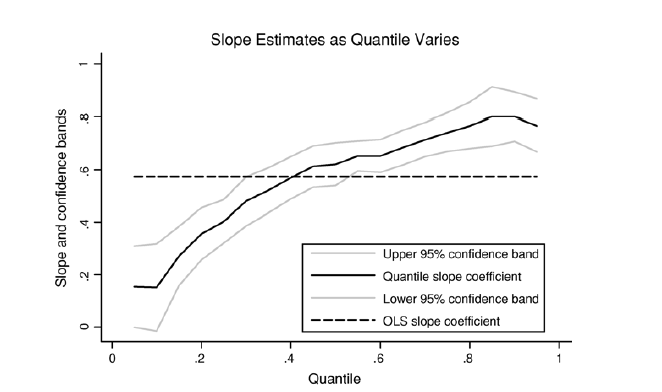
\includegraphics[keepaspectratio, width=0.8\textwidth]{qr_vietnam.png}
\end{figure}
\end{frame}

\begin{transitionframe}
  \begin{center}
         { \Huge \textcolor{white}{Nonparametric Regression}}
       \end{center}
\end{transitionframe}

\begin{frame}
\frametitle{We now let DGP be anything!}
\begin{itemize}
\item Assume that an IID data $(y_i,x_i)$ has DGP $P_0(y|X)$
\begin{itemize}
\item DGP being $E[y|X]=X\beta$: we imposed linear (in parameters) model assumption
\item We remove any modeling assumption, other than being a function of $X$, $E[y|X]=m(X)$
\end{itemize}
\item In essence, we are interested in an estimation problem involving an unknown function
\item This approach is called a \textbf{nonparametric} approach. 
\item We normally use nonparametric approach to conduct a diagnostic checking of an estimated parametric model, to conveniently display key features of the dataset in part or in whole, and to conduct an inference under very weak assumptions
\end{itemize}
\end{frame}


\begin{frame}
\frametitle{Thought experiment: Nonparametric regression in a nutshell}
\begin{itemize}
\item Discrete $Y$ and $X$
\[
\widehat{P}(y\in A| x\in B)=\frac{n^{-1}\sum_{i=1}^n\mathbb{I}(y_i\in A, x_i\in B) }{n^{-1}\sum_{i=1}^n\mathbb{I}(x_i\in B)}
\]
\item Continuous variables:  $P_0(Y\leq y|x)$
\begin{itemize}
\item $A\equiv (-\infty, y], B\equiv[x-\epsilon, x+\epsilon]$ and use $\lim_{\epsilon\to0}\widehat{P}(A|B)$ to back out the DGP
\item As $\epsilon$ becomes smaller, there are fewer points to use, leading to highly volatile estimates
\item Even more problematic when we have too many dimensions of X
\end{itemize}
\item Takeaway: 
\begin{itemize}
\item We are estimating a distribution $f$ (Kernel density estimation)
\item Interval of $X$ matters in estimation (choice of bandwidth)
\item Much more so with large $X$ dimensions (curse of dimensionality)
\end{itemize}
\end{itemize}
\end{frame}

\begin{frame}
\frametitle{Kernel density estimation}
\begin{itemize}
\item We want an estimation of $f$ that is smooth and non-negative
\item Empirical CDF won't do: It is a step function and $f=F'$ has Dirac masses
\item Kernel estimation: Idea is that we can estimate $f(y)$ by
\[
f(y)\simeq \frac{\int^{y+h}_{y-h} f(u)du}{2h}
\]
over a small interval $[y-h, y+h]$
\item Get the numerator estimates with a sample analogue
\[
\frac{1}{n}\sum_{i=1}^n \mathbb{I}\{y-h\leq y_i \leq y+h \}
\]
\end{itemize}
\end{frame}

\begin{frame}
\frametitle{Kernel density estimation: Derivation}
\begin{itemize}
\item Combining the two expressions, we can approximate $f(x)$ with
\begin{align*}
\hat{f}_n(y)&=\frac{1}{2nh}\sum_{i=1}^n \mathbb{I}[y-h\leq y_i \leq y+h]\\
&=\frac{1}{nh}\sum_{i=1}^n \frac{1}{2}\mathbb{I}\left[\left|\frac{y-y_i}{h}\right| \leq 1\right]\\
&=\frac{1}{nh}\sum_{i=1}^n K\left(\frac{y-y_i}{h}\right)\\
\end{align*}
\item Here, I use $K(u)=\frac{1}{2}1(|u|\leq 1)$. But you can use any other ones that are symmetric, nonnegative over its domain, and integrate to 1.
\item $\hat{f}_n(y)$ is the kernel density estimator for $f(y)$
\end{itemize}
\end{frame}

\begin{frame}
\frametitle{Types of kernels}
\begin{figure}[H]
\centering
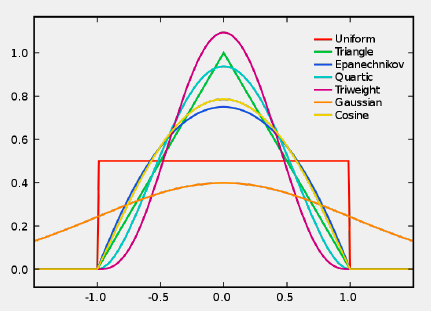
\includegraphics[width=0.6\textwidth, keepaspectratio]{kernel.png}
\end{figure}
\end{frame}

\begin{frame}
\frametitle{...but Bandwidth really matters (AKA Bart Simpson Graph)}
\begin{columns}[T]
\begin{column}{.49\textwidth}
\begin{figure}[H]
\centering
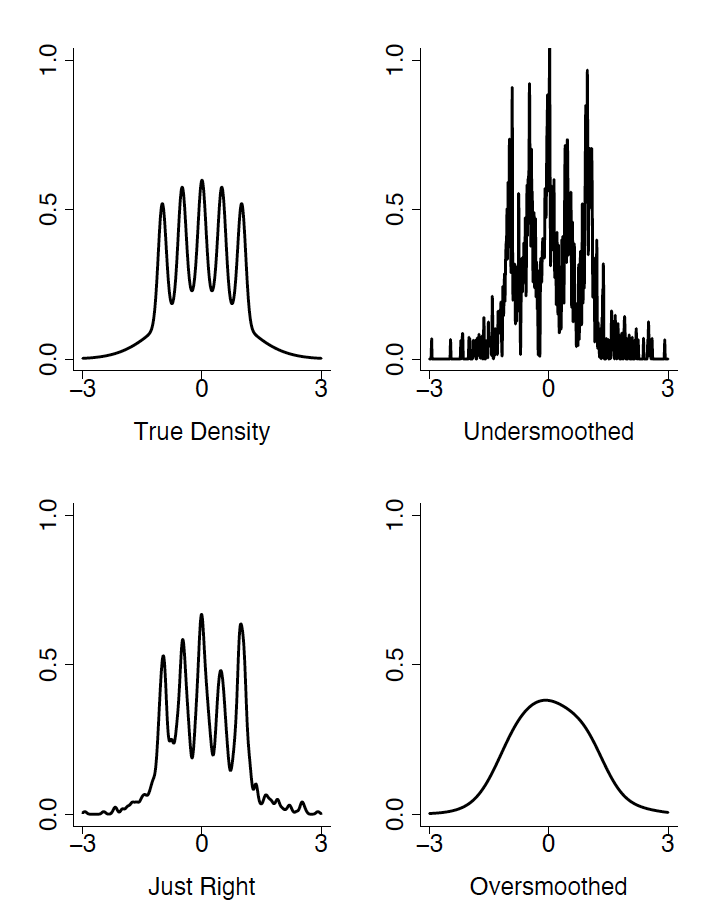
\includegraphics[width=.7\textwidth, keepaspectratio]{smoothing.png}
\end{figure}
\end{column}
\begin{column}{.49\textwidth}
\begin{itemize}
\bigskip
\item Undersmoothed: Too much volatility of $\hat{f}$ in small intervals
\bigskip
\item Oversmoothed: Lose accuracy of $\hat{f}$ in large intervals
\bigskip
\item What we have: Bias and variance move in opposite directions with respect to the length of the interval (bandwidth) $\to$ Bias-variance tradeoff!
\end{itemize}
\end{column}
\end{columns}
\end{frame}

\begin{frame}
\frametitle{This is a new problem in nonparametric setups}
\begin{itemize}
\item In parametric setups, large $n$ took care of everything!
\[
\begin{aligned}
E[(\hat{\theta}-\theta)^2]&=E[((\hat{\theta}-E[\hat{\theta}])+(E[\hat{\theta}]-\theta))^2]\\
&=E[(\hat{\theta}-E[\hat{\theta}])^2+(E[\hat{\theta}]-\theta)^2+2(\hat{\theta}-E[\hat{\theta}])(E[\hat{\theta}]-\theta)]\\
&=E[(\hat{\theta}-E[\hat{\theta}])^2]+E[(E[\hat{\theta}]-\theta)^2]+2E[(\hat{\theta}-E[\hat{\theta}])(E[\hat{\theta}]-\theta)]\\
&=\underbrace{E[(\hat{\theta}-E[\hat{\theta}])^2]}_{V(\hat{\theta})}+\underbrace{(E[\hat{\theta}]-\theta)^2}_{\text{Bias}(\hat{\theta},\theta)^2}
\end{aligned}
\]
\item Bias is $O\left(\frac{1}{n^2}\right)$ and that variance is $O\left(\frac{1}{n}\right)$
\item Increasing $n$ reduces both!
\item Nonparametrics: There is another parameter $h$....
\end{itemize}
\end{frame}

\begin{frame}
\frametitle{Smaller $h$ reduces bias... }
\begin{itemize}
\item We can write the bias as 
\footnotesize{\begin{align*}
E[\hat{f}_n(y)]&=E\left[\frac{1}{nh}\sum_{i=1}^n K\left(\frac{y-y_i}{h}\right)\right]=\frac{1}{h}\int_{-\infty}^\infty K\left(\frac{y-t}{h}\right)f(t)dt\\
&=\int_{-\infty}^\infty K(-u)f(y+uh)du \ \left(\because \frac{t-y}{h}=u \ \text{transformation, also } du=\frac{1}{h}dt\right)\\
&=\int_{-\infty}^\infty K(-u)\left[f(y)+f'(y)uh + \frac{f''(y)u^2h^2}{2}+o(h^2)\right]dt \ (\because \text{Taylor approximate around $y$}) \\
&=f(y)+0+\frac{1}{2}\int_{-\infty}^\infty K(-u)u^2h^2f''(y)du + o(h^2)
\end{align*}}\normalsize
\begin{itemize}
\item $\int_{-\infty}^\infty K(-u)du=\int_{-\infty}^\infty K(u)du=1$ by symmetry \& integrates to 1
\item Symmetry justifies $\int_{-\infty}^\infty uK(u)dt=0$ and $K(u)=K(-u)$
\end{itemize}
\item Bias: $E[\hat{f}(x)]-f(x)=\frac{1}{2}\int_{-\infty}^\infty K(u)u^2h^2f''(y)du$
\end{itemize}
\end{frame}


\begin{frame}
\frametitle{Smaller $h$ increases variance}
\begin{itemize}
\item We can write variance as
 \scriptsize{\begin{align*}
Var[\hat{f}_n(y)]&=E[\hat{f}^2(y)]-(E[\hat{f}(y)])^2\\ 
&=E\left[\frac{1}{n^2h^2}\left(\sum_{i=1}^nK\left(\frac{y-y_i}{h}\right)\right)^2\right]-(E[\hat{f}(y)])^2\\
&=E\left[\frac{1}{n^2h^2}\left(\sum_{i=1}^nK^2\left(\frac{y-y_i}{h}\right)+2\sum_{i<j} K\left(\frac{y-y_i}{h}\right)K\left(\frac{y-y_j}{h}\right)\right)\right]-(E[\hat{f}(y)])^2\\
&=\frac{1}{nh^2}\int_{-\infty}^\infty K^2\left(\frac{y-t}{h}\right)f(t)dt+\frac{n(n-1)}{n^2h^2}\left(\int_{-\infty}^\infty K\left(\frac{y-t}{h}\right)f(t)dt\right)^2-\frac{1}{h^2}\left(\int_{-\infty}^\infty K\left(\frac{y-t}{h}\right)f(t)dt\right)^2
 \end{align*}}\normalsize
\item Focusing on first term, we get (use Taylor expansion and variable transformation)
  \footnotesize{\[
 \frac{1}{nh^2}\int_{-\infty}^\infty K^2\left(\frac{y-t}{h}\right)f(t)dt=\frac{1}{nh}\int_{-\infty}^\infty K^2(-u)f(y+uh)du\simeq \frac{1}{nh}\int_{-\infty}^\infty K^2(u)f(y)du = O\left(\frac{1}{nh}\right)
 \]}\normalsize
\end{itemize}
\end{frame}

\begin{frame}
\frametitle{Choice of $h$: Minimize asymptotic mean integrated squared error}
\begin{itemize}
\item AMISE: $ \int E[\hat{f}_n(y)-f(y)]^2dy$
\item We can write $E[\hat{f}_n(y)-f(y)]^2$ as
 \footnotesize{\begin{align*}
 E[(\hat{f}_n(y)-f(y))^2] &=E[(\hat{f}_n(y)-E[\hat{f}_n(y)]+E[\hat{f}_n(y))-f(y)]^2]\\
 &=E[(\hat{f}_n(y)-E[\hat{f}_n(y)])^2+(E[\hat{f}_n(y)]-f(y))^2 +2(\hat{f}_n(y)-E[\hat{f}_n(y)])(E[\hat{f}_n(y)]-f(y))]\\
 &=E[(\hat{f}_n(y)-E[\hat{f}_n(y)])^2]+E[(E[\hat{f}_n(y)]-f(y))^2]\\
  &=\underbrace{E[(\hat{f}_n(y)-E[\hat{f}_n(y)])^2]}_{V(\hat{f}_n)(y)}+\underbrace{(E[\hat{f}_n(y)]-f(y))^2}_{\text{Bias}(\hat{f}_n(y), f(y))^2}\\
 \end{align*}}\normalsize
 \item Plug in values for bias and variance to get
    \begin{align*}
 E[(\hat{f}_n(y)-f(y))^2] =\frac{1}{nh}\int_{-\infty}^\infty K^2(u)f(y)du+\frac{h^4}{4}(f''(y))^2\left(\int_{-\infty}^\infty K(u)u^2du\right)^2
 \end{align*}
\end{itemize}
\end{frame}


\begin{frame}
\frametitle{Optimal 1-dimensional $h$}
\begin{itemize}
\item AMISE can be written as 
 \[
 \int(\text{Variance}+\text{Bias}^2)dy=\frac{1}{nh}\int_{-\infty}^\infty K^2(u)du+\frac{h^4}{4}\int_{-\infty}^\infty(f''(y))^2\left(\int_{-\infty}^\infty K(u)u^2du\right)^2 dy
 \]
 or write  $A=\frac{1}{4}\int_{-\infty}^\infty(f''(y))^2\left(\int_{-\infty}^\infty K(u)u^2du\right)^2 dy$, and let $B=\int_{-\infty}^\infty K^2(u)du$ to get
 \[
 AMISE =Ah^4+\frac{B}{nh}
 \]
\item Minimize this w.r.t $h$ to get  $h=\left(\frac{B}{4An}\right)^{1/5}$
\item Bias and standard errors are both in $n^{-2/5}$ and AMISE will be in $n^{-4/5}$ $\to$ Estimator not CAN at $n^{-1/2}$ but at slower rate
\item We also have $f''(x)$ in $A$ $\to$ several rules to select $h$ (next class)! 
\end{itemize}
\end{frame}
%%%%%%%%%%%
\end{document}
